\chapter*{Pizza Teig Wild Art}
\begin{multicols}{2}
 {\Large Zutaten}
 \begin{Zutaten}
		\item 1kg Mehl
		\item 3g Hefe
		\item 20g Salz \left(eher 25-30g\right) 
		\item 650ml Wasser \left(eher 600ml\right) 
		
		
		
		
\end{Zutaten}
\columnbreak
\addPicture{pizzaWild.jpg}
\end{multicols}

{\Large Zubereitung} \newline
\begin{addmargin}[1cm]{0cm}
	Vermengen, danach 45min bei 30°C rasten lassen.\newline
	Kugeln formen und weitere 8h bei 5-7°C rasten.\newline
	Pizzen die nicht sofort gegessen werden mit Tomatensauce bestreichen und 2-3min vorbacken.\newline
	Am besten auf Pizzastein backen.
\end{addmargin}

\begin{figure}[H]
	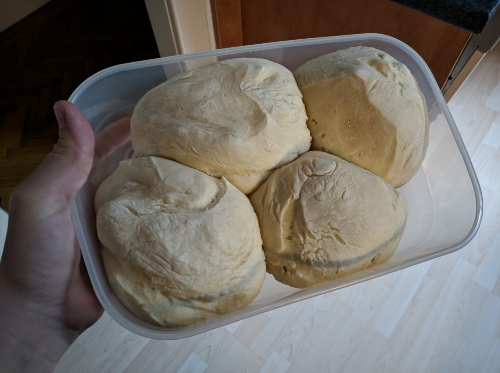
\includegraphics[width=\textwidth*0.5]{figures/pizzaWild2.jpg}
\end{figure}